
\chapter{基于动态词向量的联合嵌入模型}
视觉问答来的研究受到机器学习算法在自然语言处理和图像识别等领域成功应用的启发,因此从2015年视觉问答任务出现至今,大量的VQA模型都使用了联合嵌入模型,使之成为目前视觉问答的的主流模型。顾名思义,联合嵌入模型是将任务的源信息——图像和问题文本——表示为向量,再通过特征融合,将不同模态的信息映射到统一的向量空间,最终从联合表征中提取出答案。因为这种架构的模型易于训练,研究者采用不同的图像特征的提取方法、不同的文本特征的提取方法、两种模态的不同融合方法,做了许多尝试。

Antol等人在2015年发布了开放问题的视觉问答数据集VQA\citing{antol2015vqa}之后,在数据集的基础上提出了VQA挑战。VQA挑战中涌现了大量视觉问答模型,模型的准确率也逐年升高,图\ref{vqa_challenge}展示了2015年-2019年VQA挑战中的最优模型的准确率。通过研究其中表现优异的模型,我们发现几乎所有模型都使用了联合嵌入模型,并且加入注意力机制之后准确率能够进一步提升,例如,四年的冠军模型都是使用了注意力机制的联合嵌入模型,其中2019年的冠军模型\citing{Yu_2019_CVPR}能在VQA2.0数据集下获得总体75\%作用的准确率,相较于四年前的模型准确率得到了20\%的提升,并且距离人类表现也只有5\%左右的差距。
\begin{figure}[H]
	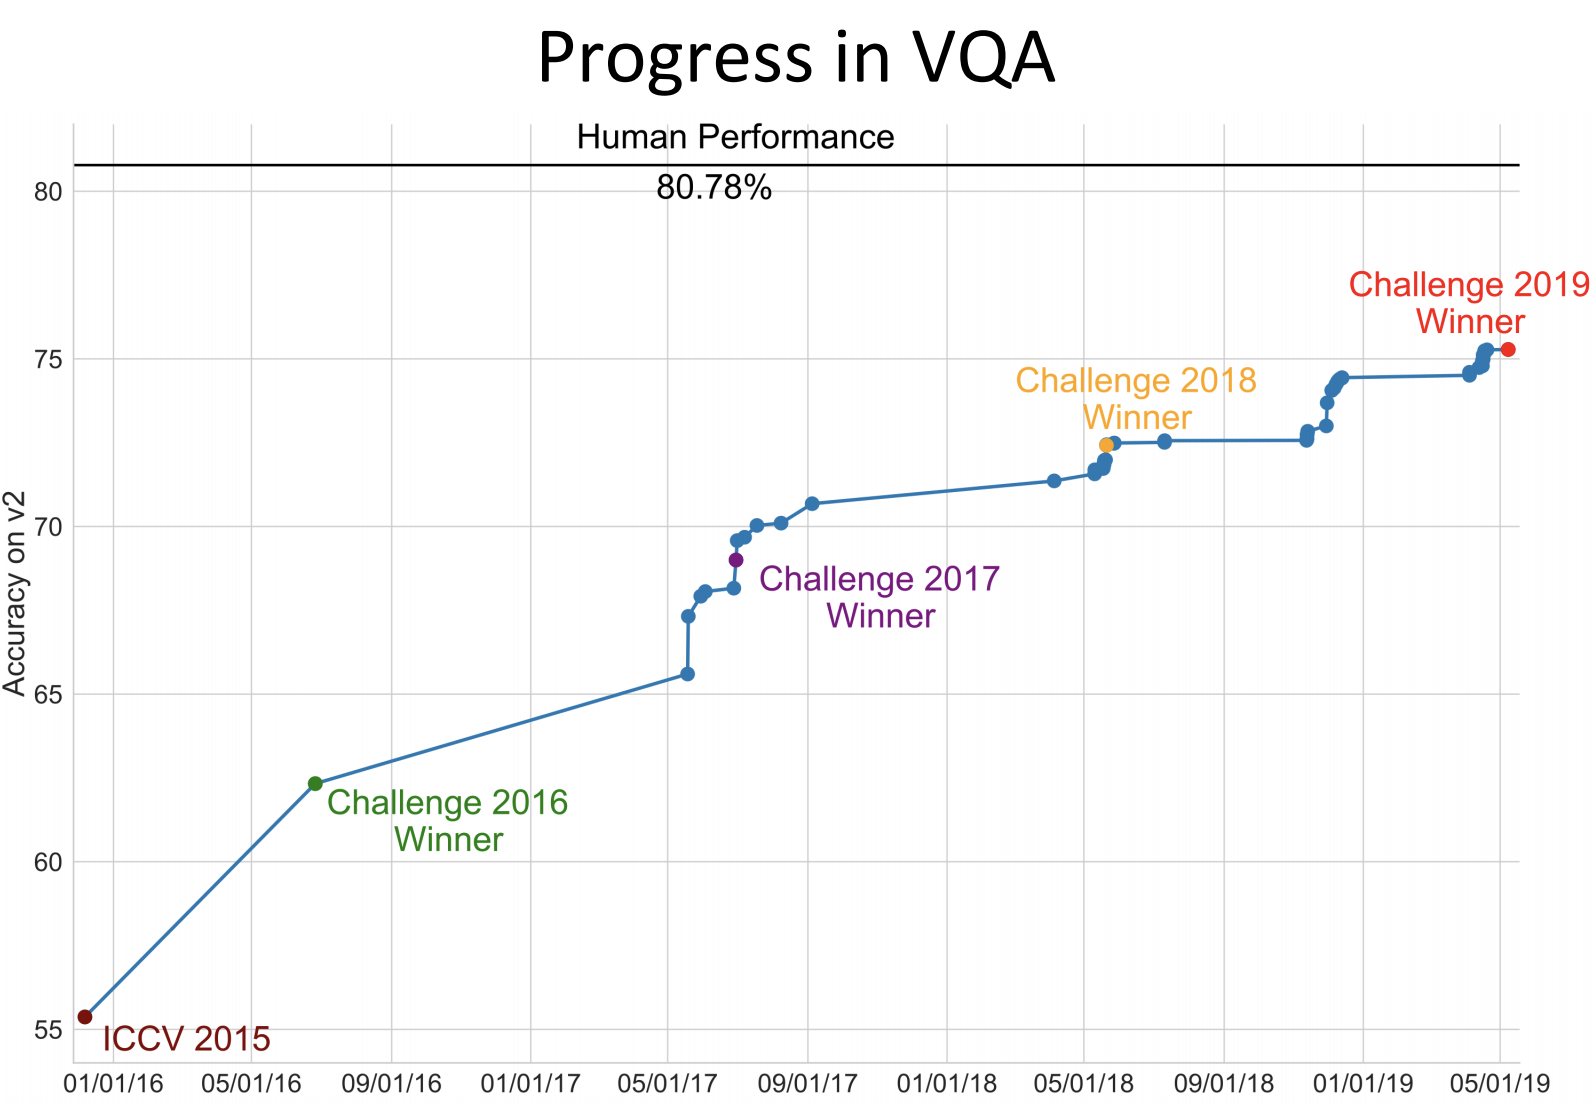
\includegraphics[width=0.7\textwidth]{vqa_challenge.png}
	\caption{VQA挑战中模型的准确率曲线}
	\label{vqa_challenge}
\end{figure}

我们认为联合嵌入模型在VQA挑战的优异表现有以下几点原因。
\begin{itemize}
  \item [1)] 
  引入注意力机制。2016年的优胜模型\citing{ilievski2016focused}提出“动态关注注意力(FDA)”模型,目的是根据问题中的关键词动态的对图像的不同区域分配带有权重的注意力,得到图像的全局特征和局部特征的结合。2017和2018年的优胜模型都使用论文\citing{anderson2018bottom}中的自上而下和自下而上的图像注意力机制,2019年的优胜模型使用了Transformer\citing{NIPS2017_7181}的多头注意力机制。注意力机制的引入能够减少无关特征的干扰,提高计算效率,并且一定程度的提高可解释性。
  \item [2)]
  VQA2.0数据集的局限性。VQA挑战以VQA2.0为数据集,然而根据我们提出的依照答案和源信息统计相关性的标准(详见表\ref{ques_type}),VQA2.0中需要常识或者外源知识的qi类型仅仅占所有问题的5.5\%\citing{wang2015explicit},这意味着回答绝大多数的问题都不需要额外的信息。然而在现实中的开放性问题中,涉及常识或者外源知识的问题广泛存在,因此VQA2.0数据集存在局限性,而这种局限性使得模型只需要关注图像和文本,因此联合嵌入模型成为了主要架构。
  \item [3)]
  得益于图像识别和自然处理模型的进步。联合嵌入模型具有灵活的组合模式,很容易从将其他任务中表现优异的模型迁移过来形成新的模型。
\end{itemize}

我们对具有代表性的联合嵌入模型,按照图像特征化方法、文本特征化方法、特征融合方法、VQA2.0的准确性、是否使用静态词向量,总结为表\ref{model_compar}。
\begin{table}[H]
% \resizebox{0.8\textwidth}{!}{}
\centering
\caption{代表性联合嵌入模型的比较}
\resizebox{\textwidth}{!}{
\begin{tabular}{llllll}
\toprule
\textbf{模型} & \textbf{图像特征化} & \textbf{文本特征化} & \textbf{特征融合} & \textbf{VQA准确率(\%)} & \textbf{静态词向量} \\
\midrule
LSTM Q+I \citing{antol2015vqa}&  VGGnet& LSTM&  逐项点乘&  54.1& 是\\
iBOWIMG\citing{zhou2015simple}&  GoogleNet& 词袋模型&  串联&  55.9& 是\\
DPPNet \citing{noh2016image}&  VGGnet& GRU&  动态参数层&  57.4& 是\\
D-CNN\citing{ma2016learning}&  CNN& CNN&  CNN&  58.4& 是\\
MCB\citing{fukui2016multimodal}&  RestNet& LSTM&  MCB&  64.2& 是\\
2017-winer\citing{teney2018tips}&  Faster R-CNN& Glove+GRU&  逐项点乘& 69.87 & 是\\
2018-winer\citing{anderson2018bottom}&  Faster R-CNN& Glove+GRU&  逐项点乘& 72.27 & 是\\
2019-winer\citing{Yu_2019_CVPR}&  Faster R-CNN& Glove+LSTM&  MLP& 75.26 & 是\\
\bottomrule
\end{tabular}}
\label{model_compar}
\end{table}

如上表所示,现有的联合嵌入模型采用了不同的图像特征化、文本特征化、特征融合方法的组合,但是所有现有的模型的文本特征化均使用静态词向量。静态词向量使用一个语料库作为数据集,训练得到每个词语的分布式表示,这种表示方法的优点在于词语的向量预先训练得到,因此应用于不同的下游任务时,无需再训练,提高了运算效率。然而在真实的语言环境中,同一词语在不同的语境中表示不同的含义,也可能作为不同的语法成分,而这些差异并不能被静态词向量表示,因此可能出现语义和语法的偏差。

为了解决静态词向量的问题,我们构建了一个基于动态词向量的联合嵌入模型——None KB-Specific Network(N-KBSN)模型。本章将重点介绍N-KBSN模型,并且使用VQA2.0数据集训练。N-KBSN由三个主要部分组成:问题文本和图像特征提取模块、自注意力和引导注意力模块、特征融合和分类器。其中,图像特征提取使用在多目标检测中表现优秀的Faster R-CNN\citing{ren2015faster},问题文本特征提取使用能够获得上下文信息的ELMo模型\citing{Peters:2018},并使用从Transformer中借鉴的多头注意力机制\citing{NIPS2017_7181}分别实现图片的自注意力(V-SA)、问题文本的自注意力(Q-SA)、由问题引导的对图像的注意力(Guided Attention, GA),最后通过特征融合预测答案。N-KBSN模型的基础架构如图\ref{N-KBSN}。
\begin{figure}[H]
	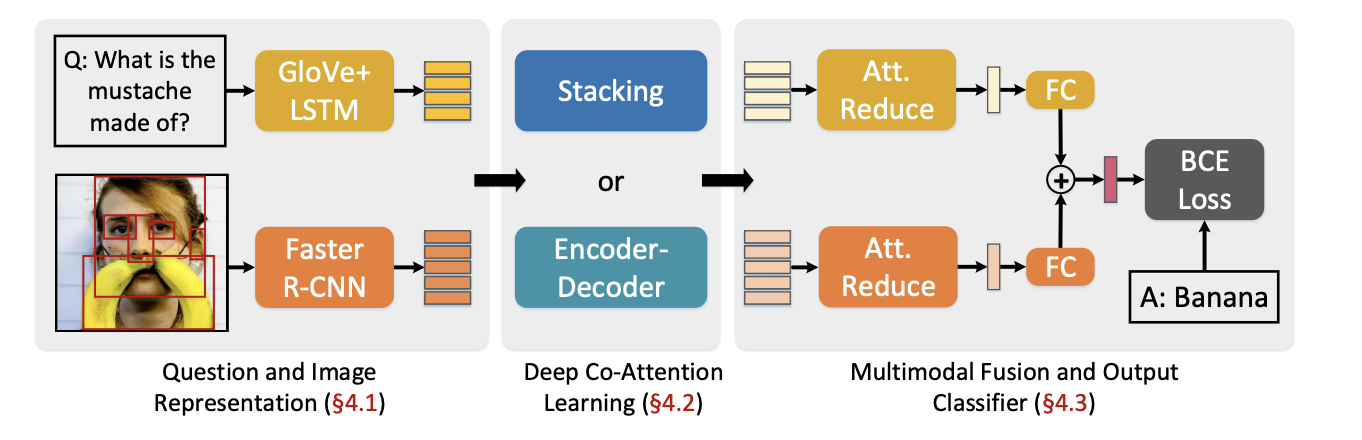
\includegraphics[width=0.8\textwidth]{N-KBSN.png}
	\caption{N-KBSN基础结构}
	\label{N-KBSN}
\end{figure}

\section{基于Faster R-CNN的图像特征化}
目标检测是机器视觉领域的重要应用之一,目标检测的核心任务是准确、快速的从图像中定位出目标并且能识别目标的类别、属性等特性。传统的目标检测算法通过滑动窗口的方式选取区域选择、提取特征提并分类,例如可变形的组件模型(DPM)方法\citing{felzenszwalb2009object}等。这些传统的目标检测算法大多区域选择的策略效果差、时间复杂度高,并且因为由于是人工提取特征,提取的特征层次较低,致使模型的鲁棒性较差。由于深度学习在视觉问答任务的优异表现,大批优秀的目标检测算法出现,例如R-CNN\citing{girshick2014rich}、SPP-Net\citing{he2015spatial}、Fast R-CNN\citing{girshick2015fast}、Faster R-CNN\citing{ren2015faster}、Mask R-CNN\citing{he2017mask}、YOLO\citing{redmon2016you}及其后续版本等。以上的模型大致分为两个主要类别,第一类为两阶段检测模型,由候选区域识别和区域特征提取组成,例如R-CNN系列模型;第二类为单阶段检测模型,使用端对端的训练,不添加候选区域识别的网络,例如YOLO系列模型。由于Faster R-CNN在各个目标识别任务的出色表现,本节将省略对单级式检测框架的介绍,并着重介绍本文中图像处理的核心模型Faster R-CNN。

不同于传统目标检测模型使用的的滑动卷积窗口,R-CNN 采用选择性搜索的方法来预先提取一些可能包含目标物体的候选区域(region proposal),再使用卷积神经网络提取各个图像区域的特征,再将提取的特征送入SVM分类器完成类别识别,最后使用回归器对目标位置进行修正。这种方法显著的提升识别速度,降低了计算成本,也提高了准确率。但由于候选区域的提取是相互独立的,因此可能存在像素重叠,使得R-CNN会对同一区域重复提取特征。为了减少R-CNN的重复计算,研究者提出了SPP-Net。该算法使用空间金字塔池化层(Spatial Pyramid Pooling)裁剪和缩放候选区域,使得图像大小一致,再输入到卷积层进行特征提取。随后的Fast R-CNN借用了SPP-Net的空间金字塔池化层,设计了兴趣区域池化(RoI Pooling),将图像中的多个兴趣区域池化成相同大小的特征图,并使用这些特征图同时预测物体类别和框出对象的区域。这种方法解决了输入候选区域尺寸不一致的问题,并且提高了计算速度。但是Fast R-CNN在生成生成候选区域的较慢,为了解决这一问题,R-CNN的作者又提出了Faster R-CNN。

Faster R-CNN同样沿袭了先前R-CNN和Fast R-CNN的两阶段检测框架,并构建了一个筛选候选区域的网络(Region Proposal Network, RPN),用于控制候选区域的数量。该网络将CNN处理后的全局图像特征作为输入,输出候选区域,最终的分类器结合全局的图像特征和候选区域预测各个区域的类别。
\begin{figure}[H]
	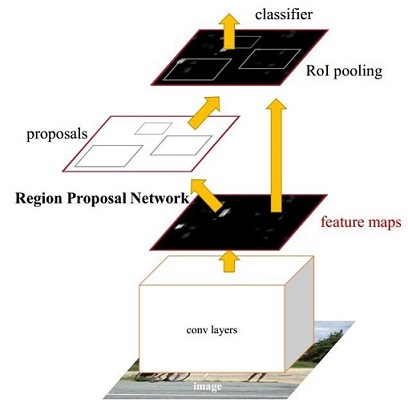
\includegraphics[width=0.5\textwidth]{Faster_R_CNN.png}
	\caption{Faster R-CNN基本结构}
	\label{Faster_R_CNN}
\end{figure}

如图\ref{Faster_R_CNN},Faster R-CNN可以根据功能的不同将模型分为四个模块:卷积层、区域候选网络(RPN)、兴趣区域池化(RoI Pooling)、分类器。卷积层使用CNN及其变型提取图像特征,生成的特征图被共享用于后续RPN层和全连接层,这种对图像的处理方式不同于R-CNN和Fast R-CNN。后两者都是先从原始图像中提取候选区域,再分别对候选区域提取特征。RPN网络用于预测候选区域,该网络在CNN输出的图像特征上滑动,在每个空间区域,网络都会预测类别得分,兴趣区域池化层结合图像的特征图和候选区域,得到区域特征图,再使用全连接层和分类器,预测每个区域的类别,同时利用候选框回归得到对象的检测框。

在本文中,我们使用联合在ImagNet\citing{russakovsky2015imagenet}上预训练的ResNet-101和在Visual Genome\citing{krishna2017visual}上预训练Faster R-CNN提取图像特征。给定图像$I$,我们从图像中提取$m$个大小不固定的图像特征,$X=\{x_1, x_2, ..., x_m\}, x_i \in \mathbb{R}^D$,每一个图像特征编码一个图像区域。每个图像区域的特征图维度为2048。对卷积层输出的特征图,我们使用非极大抑制(non-maximum suppression)和单元重合(IoU)阈值筛选出排名靠前的候选区域,通过设定一个目标检测概率的阈值,我们获得一个动态的被检测对象的数量$m \in [10,100]$,并且使用零填充使得$m=100$。对于每个所选区域$i$,$x_i$被定义为该区域的特征图的均值池化结果,并将$m$个区域的$x_i$拼接成为最终的图像特征。因此,每一张输入的图像将会被转化为一个$100\times 2048$的图像特征,供后续的注意力模块使用。

\section{基于ELMo的文本特征化}

如表\ref{model_compar}所示,以往的视觉问答模型的文本特征化都是通过对语料库的学习得到静态的词向量,即每个单词对应一个确定的实数向量,这种固定向量在处理词汇的多义性上表现不佳。无论是中文词语还是英文单词都广泛得存在一词多义的现象,即同一个词在不同的语境下含义发生变化,例如,在中文中,“他正在算账”和“下回找你算账”中的“算账”由于文化演化而产生了更复杂的引申义,又如英文中的“where is the bank?”和“It is the bank of the river”中的“bank”在第一句中译为“银行”而第二句中译为“河畔”。为解决一词多义的问题,研究者提出了动态词向量,ELMo和BERT便是其中的代表。ELMo在多个NLP任务中均提高了模型的准确率,因此本文将引入ELMo模型处理视觉问答任务中的文本,并在后续的处理中结合类似于BERT的注意力机制。

ELMo模型是一种能感知上下文的词向量生成模型,其模型深度能够有效建模词语复杂的语义和语法,能根据词语的上下文生成动态向量,进而为解决一词多义和一词多用提供了可能。ELMo采用了两个阶段获得词向量,第一个阶段是用大量的文本语料训练一个深度双向语言模型(biLSTM);第二个阶段从预训练网络中提取对应单词的网络各层的内部状态(internal state),并通过函数转化为词向量。ELMo模型的结构如图\ref{elmo}。
\begin{figure}[H]
	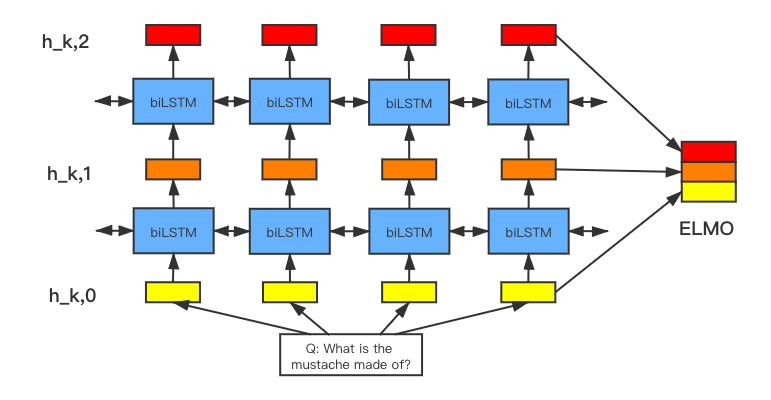
\includegraphics[width=0.8\textwidth]{elmo.png}
	\caption{ELMo模型架构}
	\label{elmo}
\end{figure}

语言模型是对语句的概率分布的建模。语言模型分为前向和后向,前向是指已知上文的词语,推理下一个词语的方式,而后向则是已知后文的内容,求解上一个词语的方式。对于一个具有N个单词的句子$S=(t_1, t_2, ..., t_N)$而言,前向语言模型就是求解以下公式的最大值:
\begin{equation}
p(t_1, t_2, ..., t_N)=\prod_{k=1}^N p(t_k|t_1,t_2,...,t_{k-1})
\end{equation}
其中$p(t_1, t_2, ..., t_N)$为序列的联合概率,
$p(t_k|t_1, t_2,..., t_{k-1})$表示已知$t_k$的上文$(t_1, t_2, ..., t_{k-1})$的条件下,求解$t_k$的条件概率。对应的后向语言模型的公式为
\begin{equation}
p(t_1, t_2, ..., t_N)=\prod_{k=1}^N p(t_k|t_{k+1},t_{k+2},...,t_N)
\end{equation}

ELMo使用双向LSTM(biLSTM)模型作为语言模型的基础。首先将“上下文无关的”初始词向量$y{_k^{LM}}$输入L层的前向LSTM。在位置k上,LSTM将输出一个“上下文相关”的词表征$\vec{h}_{k,j}^{LM,j}$,其中$j = 1, ..., L$。最后一层的LSTM输出$\vec{h}_{k,j}^{LM,L}$通过一个softmax层预测下一个词语的初始词向量$y{_{k+1}^{LM}}$。后向LSTM类似于前向LSTM有L层并且在k位置上得到一个词表征$\overleftarrow{h}_{k,j}^{LM}$。最后通过最大似然的方式训练双向LSTM模型,公式如下:
\begin{equation}
\sum_{k=1}^N(\log_p(t_k|t_1, t_2,..., t_{k-1};\Theta_x,\overrightarrow{\Theta_{LSTM}},\Theta_s) + \log_p(t_k|t_{k+1},t_{k+2},...,t_N;\Theta_x,\overleftarrow{\Theta_{LSTM}},\Theta_s)
)
\end{equation}

其中,$\Theta_x$和$\Theta_s$分别是训练阶段时的两个softmax层的参数,$\overrightarrow{\Theta_{LSTM}}$和$\overleftarrow{\Theta_{LSTM}}$是biLSTM的参数。

,完成预训练的模型对输入句子的每个单词输出三种Embedding:最底层是初始的词向量$y{_k^{LM}}$;前向LSTM输出的$\overrightarrow{h}_{k,j}^{LM}$;后向LSTM输出的$\overleftarrow{h}_{k,j}^{LM}$。ELMo将三种词向量串联,得到
\begin{equation}
R_k = 
[y_k^{LM}, \overrightarrow{h}_{k,j}^{LM}, \overleftarrow{h}_{k,j}^{LM} | j = 1, ..., L]
= [h_{k,j}^{LM} | j = 0, ..., L]
\end{equation}

其中$h_{k,0}^{LM}$是初始词向量,$h_{k,j}^{LM} = [\overrightarrow{h}_{k,j}^{LM}; \overleftarrow{h}_{k,j}^{LM}]$ 是每个biLSTM层输出的结果。

最后使用以下公式得到对应单词的具有”上下文信息“的词向量。
\begin{equation}
ELMo_k^{task} = E(R_k; \Theta^{task}) = \gamma^{task}\sum_{j=0}^L s_j^{task} h_{k,j}^{LM}
\end{equation}

其中是$s_j^{task}$任务相关训练得到的权重参数, $\gamma$是一个任务相关的scale参数。

在本文中,我们将句子最大长度裁剪为14个,并使用零填充的方式将不足14个词的句子补足为14,即$n=14$。并将每个单词转化为50维的初始词向量,即$y_k^{LM}\in \mathbb{R}^{50}$。假定双向语言模型的层数为$L = 2$,隐层节点数为$H_{dim}$,输出维度为$output_{dim} \in \mathbb{R}^d$,则$ELMo_k^{task} \in \mathbb{R}^{2d}$,输出的文本特征$Y \in \mathbb{R}^{n\times 2d}$。

\section{基于多头注意力机制的特征增强}
正如绪论中提到的,注意力机制的引入帮助神经网络提高了预测精度,并且减少了计算复杂度。视觉问答任务由于需要处理多模态的数据——图像和文本,比起仅需要处理单模态的数据的任务更需要进行高效的计算。同时,VQA任务输入的图像和问题文本具有高度的相关性,因此两种模态的数据之间的交互对于结果的准确性的提升也具有显著的影响。对于以上两个需求,我们在N-KBSN中使用了Transformer\citing{NIPS2017_7181}的多头注意力机制(Multi-head Attention, MA)实现图片的自注意力(V-SA)、问题文本的自注意力(Q-SA)、由问题引导的对图像的注意力(Guided Attention, GA)。

注意力机制本质上是找到一个方式对已有信息分配合适的权重,并以此提高输出的准确性。我们可以将注意力函数描述成映射查询(query)到一些键值对(key-value pair)并由此得到输出。假定查询矩阵$Q = \{q_1, q_2, ..., q_m\}$,其中查询向量$q_i \in \mathbb{R}^{1 \times d_q}$;key矩阵$K = \{k_1, k_2, ..., k_n\}$,其中$k_j\in \mathbb{R}^{1 \times d_k}$;value矩阵$V = \{v_1, v_2, ..., v_n\}$,其中value向量$v_i \in \mathbb{R}^{1 \times d_v}$,那么注意力特征可以通过对value矩阵的加权得到,权重可以通过查询矩阵和key矩阵得到:
\begin{equation}
Attention(Q, K, V) = score(Q, K)V
\end{equation}
其中$score(Q, K)$为计算权重的函数,有多种计算方式,本文使用Transformer中的缩放点乘法:
\begin{equation}
score(Q, K) = softmax(\frac{QK^T}{\sqrt{d_k}})
\end{equation}
其中$q_i$和$k_j$要求具有相同的维度。
因此可以得到:
\begin{equation}
Attention(Q, K, V) = softmax(\frac{QK^T}{\sqrt{d_k}})V
\end{equation}

为了进一步提高注意力特征的表达能力,引入多头注意力机制。多头注意力机制的实现过程是,将上式的$Q, K, V$输入到$h$个具有不同权重的线性层,得到$(Q_i, K_i, V_i), i = 1, 2, ..., h$,再分别计算得到$Attention(Q_i, K_i, V_i), i = 1, 2, ..., h$,最后将$h$个注意力特征拼接并通过一个线性层获得期望维度的注意力特征,如图\ref{ma}。多头注意力机制的公式为:
\begin{equation}
MA(Q, K, V) = [head_1, head_2, ..., head_h]W
\end{equation}
\begin{equation}
head_i = Attention(Q_i, K_i, V_i)
\end{equation}
其中$W$为线性层的权重。
\begin{figure}[H]
	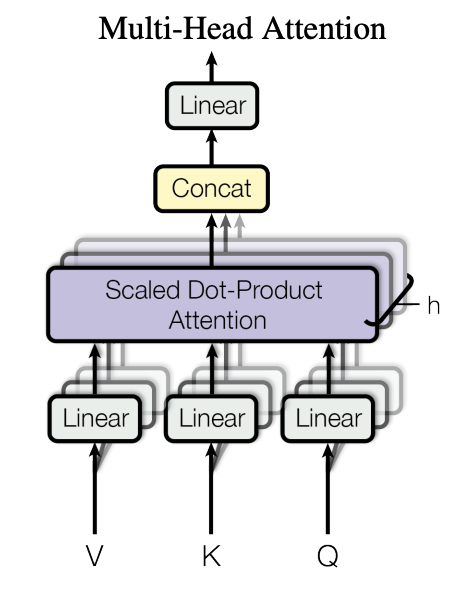
\includegraphics[width=0.5\textwidth]{ma.png}
	\caption{多头注意力的架构}
	\label{ma}
\end{figure}

基于以上多头注意力机制的思想,本文分别使用三种注意力特征:图片的自注意力(V-SA)、问题文本的自注意力(Q-SA)、由问题引导的对图像的注意力(GA)。假设文本词向量矩阵为$Y$,图像特征图为$X$,则在计算V-SA时,$Q = K = V = X$,即输出的图像特征为$SA=MA(X, X, X)$;在计算Q-SA时,$Q = K = V = Y$,即输出的文本特征为$SA=MA(Y, Y, Y)$;在计算引导注意力特征时,$Q = Y$为词向量矩阵,$K = V = X$为图像特征矩阵,并且词向量和图像特征向量具有相同的维度,即输出的由问题引导的图像特征为$GA=MA(Y, X, X)$。三种注意力组合的结构构成一个共同注意力模块(MCA),结构如图\ref{mca}。共同注意力模块以输入为原始的图像特征和文本特征,输出为经过注意力机制的图像和文本特征。
\begin{figure}[H]
	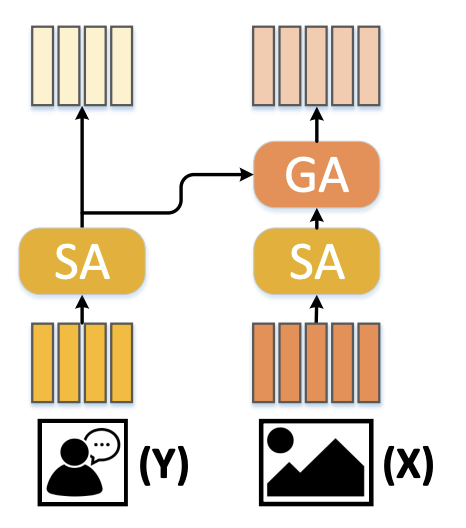
\includegraphics[width=0.3\textwidth]{mca.png}
	\caption{共同注意力模块结构}
	\label{mca}
\end{figure}

为了提高使用深度的注意力机制提取更高层次的特征,MCAN论文\citing{Yu_2019_CVPR}提出了Encoder-Decoder和Stacking两种级联MCA层的方式,如图\ref{mca_stacking}。其中,Stacking将上一层的输出直接作为下一层的输入,Encoder-Decoder将最后一层的问题自注意力特征作为每一层图像的查询矩阵。
\begin{figure}[H]
	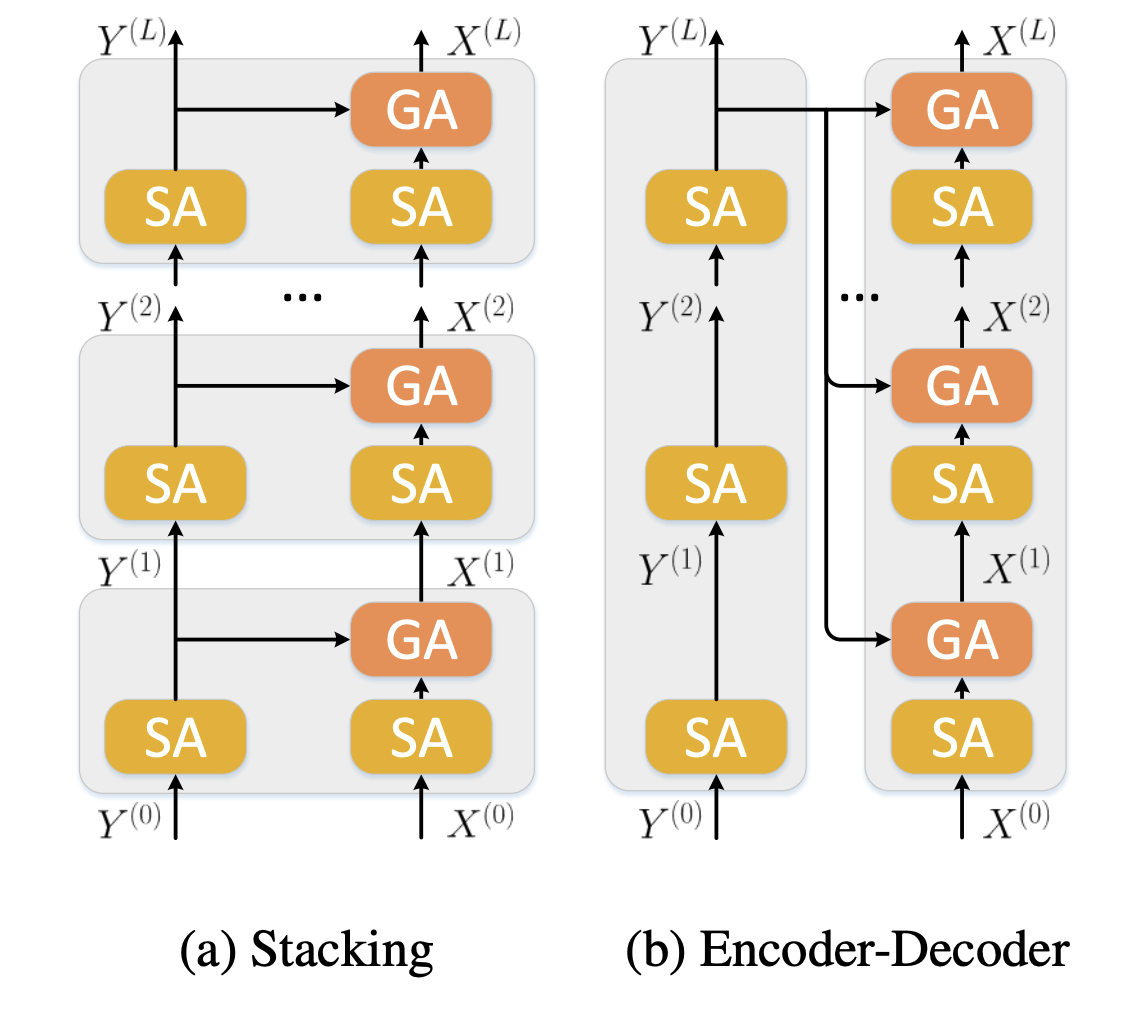
\includegraphics[width=0.5\textwidth]{mca_stacking.png}
	\caption{两种MCA层的级联方式}
	\label{mca_stacking}
\end{figure}

根据文章给出的两种级联方式在多个任务的表现情况\citing{Yu_2019_CVPR},在本文中,我们使用Encoder-Decoder的级联方式,假定$SA^1$,$SA^2$,...,$SA^L$表示不同层的自注意力,$GA^1$,$GA^2$,...,$GA^L$表示不同层的引导注意力,$X^{(k)}$和$Y^{(k)}$分别表示第k层输出的图像特征和文本特征。因此第k层Encoder-Decoder级联的注意力模块的公式为,
\begin{equation}
Y^{(k)} = SA^{(k)}(Y^{(k-1)})
\end{equation}
\begin{equation}
X^{(k)} = GA^{(k)}(Y^{(L)}, SA^{(k)}(X^{(k-1)}))
\end{equation}
其中图像特征$X^{(0)}=X$,$Y^{(0)}=Y$。

在获得经过多层注意力的图像特征$X^{(L)}=[x^{(L)}_1,...,x^{(L)}_m]\in\mathbb{R}^{m \times d}$和文本特征$Y^{(L)}=[y^{(L)}_1,...,y^{(L)}_n]\in\mathbb{R}^{n \times d}$,我们对所有分量权重求和,进一步得到最终的图像特征$x$和文本特征$y$。以图像特征为例,公式如下。
\begin{equation}
\alpha = softmax(MLP(X^{(L)}))
\end{equation}
\begin{equation}
x = \sum_{i=1}^m \alpha_i x_i^{(L)}
\end{equation}
其中$\alpha = [\alpha_1,...,\alpha_m]$是图像特征分量的权重。

$Y^{(L)}$的计算方式类似。我们使用一下公式融合两种特征。
\begin{equation}
z = LayerNorm(W_x^Tx + W_y^Ty)
\end{equation}
其中$W_x, W_y \in \mathbb{R}^{d \times d_z}$是线性映射矩阵,$d_z$是融合后的特征向量的维度。最后我们使用softmax函数计算融合特征在$N$个类别的答案,$N$为训练集中出现频率最高的答案。最后我们使用交叉熵更新模型参数。

\section{实验}
本节将构建一系列有不同网络结构或者参数设置的视觉问答模型,并使用通用的开放型问答数据集VQA2.0\citing{goyal2017making}训练和评估模型。实验的目的是为了对比动态词向量和静态词向量对结果准确率的影响,并通过大量实验找到超参数最优的N-KBSN模型。整体代码使用Python实现,以pytorch为机器学习平台,并使用带有32G内存和GPU的计算机训练模型。

\subsection{实验设置}
\textbf{数据集}

我们使用VQA2.0数据集训练模型,数据集被划分为train/val/test三个数据子集,它们分别包含8万图像+44.4万问答对、4万图像+21.4万问答对、8万图像+44.8万问答对。答案包含“是否”、“数量”和“其他”三种类型,图片均为从MS-COCO数据集中提取的真实场景。此外,根据同时存在于VQA2.0和Visual Genome中的图片,我们还使用了从Visual Genome中提取出49万个问答对,用于增强训练集。

\textbf{评估方式}

为了实现对复杂推理的训练和测试,VQA2.0数据集在问题设置上采用了人工的方式,每张图片都有3个人类提出的问题。答案全为开放式问题,开放式答案的评估方法也引入人工评估机制:对于同一个开放性问题由十个人分别作答,如果有三个及以上的被测者均提供了同一答案,该答案被视为正确答案。
因此文本使用正确率作为评价参数,包括总体正确率和子项正确率。子项正确率根据答案类型分为是否、计数和其他。

\textbf{固定模块的参数设置}

本节的实验目的是对比不同的词向量嵌入策略对于模型的准确率的影响,因此模型的其他部分因保持相同的参数设置。具体来说,对于图像特征提取模块,Faster R-CNN的候选图像区域数$m = 100$,单个图像区域的特征维度$x_i = 2048$,因此单张图像特征$X \in \mathbb{R}^{100 \times 2048}$。自注意力和引导注意力模块中使用的多头注意力隐层维度$d=512$,头数$h=8$,即每个头的隐层维度$d_h=d/h=64$,MCA层数$L=6$。我们从所有答案中筛选出出现次数大于8的单词或词组,构建得到大小为$N=3129$答案词典,即分类的类别数为3129。

激活函数使用ReLU。Adam优化器参数为$\beta_1=0.9$、$\beta_2=0.98$,学习率为$min(2.5te^{-5}, 1e^{-4})$,其中t为训练的epoch数,从第10代开始,每过两代学习率衰减为当前的1/5。批样本数$batch = 32$,训练代数$epoch=13$。

\textbf{静态词向量 vs. 动态词向量}

在固定模型的其他部分不变的情况下, 我们将使用不同的本文特征化方法,以评估动态和静态词向量对于结果准确率的影响。我们选取了静态词向量中具有代表性、并且被广泛应用的预训练的word2vec和Glove词向量,并且级联一个单层的LSTM网络,将其特征维度转换为512维,便于后续和图像特征的融合。其中word2vec词向量使用的是word2vec模型在包含1000亿个单词和词组的Google News上训练得到的词向量。word2vec词向量是由表示300万个单词和词组的300维向量组成。Glove词向量是从Wikipedia和Twitter等语料库中训练得到,包含200万个300维的向量。为了使用静态词向量,我们首先输入样本的问题文本裁剪为长度为14的单词序列,再使用查找表得到每个单词的静态向量。对于数据集中不存在预训练词向量的单词,我们将其词向量初始化为零向量。

不同于静态向量的配置方式,为获得动态词向量,我们将预训练的深度双向LSTM网络(biLSTM)嵌入到模型中,并通过训练得到Elmo词向量的权重参数和尺度参数。为了进一步探究最佳的Elmo参数,我们选用了三种不同参数的预训练ELMO模型,分别是$ELMO_s$/$ELMO_m$/$ELMO_l$,它们的参数量、LSTM的隐层大小、输出大小、$ELMo_k^{task}$大小见表\ref{ELMO_models}。如表所示,三种不同参数的Elmo模型主要差异在于模型深度和词向量的维度,理论上来说,更深的网络深度具有更大的容量,并且高维的词向量能包含更多的语义信息。我们同样将问题文本裁剪为14个单词序列,并将整个单词序列作为输入,通过两层的biLSTM网络,得到包含上下文语境的Elmo词向量。我们同样使用一个LSTM网络将Elmo词向量统一转化为512维,融合特征$z \in \mathbb{R}^{1024}$。
\begin{table}[H]
% \resizebox{0.8\textwidth}{!}{}
\centering
\caption{三种 ELMO 的参数配置。}
\begin{tabular}{ccccc}
\toprule
\textbf{Model} & \textbf{Parameters (Millions)} & \textbf{LSTM Size} & \textbf{Output Size} & \textbf{ELMO Size}\\
\midrule
$ELMO_s$&  13.6& 1024&  128& 256\\
$ELMO_m$&  28.0& 2048&  256& 512\\
$ELMO_l$&  93.6& 4096&  512& 1024\\
\bottomrule
\end{tabular}
\label{ELMO_models}
\end{table}

几种词向量的统计信息如表\ref{embedding_compare}。其中,由于Elmo模型使用字符级别的编码,因此即使对于语料库中不存在的单词,仍然可以获得其初始词向量,进而得到其Elmo词向量,因此Elmo词向量的数量理论上无限。为了方便实验结果的分析,我们将配置了不同文本特征的模型分别表示为:$baseline(w2v)$, $baseline(glove)$, $N-KBSN(s)$, $N-KBSN(m)$, $N-KBSN(l)$。
\begin{table}[H]
% \resizebox{0.8\textwidth}{!}{}
\centering
\caption{word2vec, Glove, 三种elmo模型的统计信息。}
\begin{tabular}{c|c|c|c}
\toprule
\textbf{名称} & \textbf{预训练语料库(大小)} & \textbf{词向量维度} & \textbf{词向量数量} \\
\midrule
word2vec&  Google News(1000亿单词)& 300&  300万\\
Glove&  Wikipedia 2014 + Gigaword 5(60亿单词)& 300&  40万\\
\midrule
$ELMO_s$&  \multirow{3}{*}{WMT 2011(8亿单词)}& 256& \multirow{3}{*}{/}\\
$ELMO_m$&  & 512&  \\
$ELMO_l$&  & 1024&  \\
\bottomrule
\end{tabular}
\label{embedding_compare}
\end{table}

\subsection{实验结果及分析}

\subsubsection{VQA实验结果分析}

在本次的实验中,我们将使用VQA2.0数据集训练和评估六个模型,分别是$baseline(random)$, $baseline(w2v)$, $baseline(glove)$, $N-KBSN(s)$, $N-KBSN(m)$, $N-KBSN(l)$。其中$baseline(random)$的词向量使用随机初始化,并级联LSTM网络。同时,在模型对比中,我们也加入往年在VQA挑战中取得优胜的模型,$2017-winner(glove)$和$2019-winner(glove)$。各个模型在val验证集上的实验结果如表\ref{5mresults}。
\begin{table}[H]
% \resizebox{0.8\textwidth}{!}{}
\centering
\caption{使用不同文本特征化的模型在val数据集的结果。结果包括总体正确率以及三种答案类型:是否、计数、其他的单项正确率。}
\begin{tabular}{c|cccc}
\toprule
模型 & 总体正确率 & 是否 & 计数 & 其他\\
\midrule
$baseline(random)$& 62.34 &  78.77 & 41.92 & 55.27\\
$2017-winner(glove)$ & 63.22 & 80.07 & 42.87 & 55.81\\
$baseline(w2v)$&  64.37 &  81.89 &  44.51 & 56.31\\
$baseline(glove)$&  66.73 & 84.56 &  49.52 & 57.72\\
$2019-winner(glove)$& 67.22 & 84.80 & 49.30 & 58.60\\
\midrule
$N-KBSN(s)$&  67.27& 84.76&  49.31& 58.73\\
$N-KBSN(m)$&  67.55& 85.03&  49.62& 59.01\\
$N-KBSN(l)$&  \textbf{67.72}& \textbf{85.22}&  \textbf{49.63}& \textbf{59.20}\\
\bottomrule
\end{tabular}
\label{5mresults}
\end{table}

如表所示,从答案类型单项的准确率方面看,所有模型的实验结果都表现为,是否>其他>计数,且任意两个单项的准确率差值在不同模型的结果中保持稳定,这说明这种单项的准确率差异与模型无关,来源于问题本身和数据集的特性,例如,答案为是否的样本的随机猜测的期望准确率为50\%,而计数类型的随机猜测准确率很低,两种答案类型本身的难度差异导致了是否类型的准确率始终远远高于计数类型。

前五个模型均使用静态词向量作为文本特征,$baseline(random)$由于使用随机初始化的文本特征,词向量能包含的语义和语法信息相较于预训练词向量更少,因此其各项准确率均为最低。$2017-winner(glove)$由于使用更为简单的注意力机制,因此准确率低于本文的baseline模型。对比$baseline(w2v)$和$baseline(glove)$的实验结果,我们可以看出,即使word2vec词向量的语料库接近20倍于glove词向量的语料库,基于glove的模型还是呈现出全面的领先,在其他部分相同的情况下。分析其原因,正如论文\cite{pennington2014glove}所说,glove词向量使用了共现矩阵,相较于word2vec只使用局部的上下文信息,引入了语料库的全局信息,提高了表征能力,因此,即使使用了更大的语料库训练得到的word2vec词向量表征能力依然差于glove。

最后三个模型是本文提出的N-KBSN模型,从结果可以看出,对比$baseline(glove)$,各项的准确率均有显著提升,这证明了动态词向量确实能一定程度的提高模型的文本表示能力,进而提高整体的结果准确率。而对比三种不同参数的elmo模型,我们发现,随着模型深度和特征维度的提高,整体的准确率并没有特别明显的提高。具体来说,$N-KBSN(l)$的elmo模型参数量是$N-KBSN(m)$的三倍多,但是准确率并无明显提升。我们选用$N-KBSN(l)$作为参考模型,供之后的基于知识库图嵌入的KBSN模型使用。

如表\ref{5mresults}所呈现出的结果,使用了Elmo动态向量的N-KBSN模型的实验结果全面优于使用Glove静态词向量的$baseline(glove)$。为了进一步探究其原因,我们以$N-KBSN(m)$和$baseline(glove)$作为实验模型,进行了定量分析和定性分析。

\subsubsection{定量分析}
为了定量分析$N-KBSN(m)$和$baseline(glove)$的差异,我们将VQA2.0的train随机采样,分别构成大小为原始大小10\%, 30\%, 50\%, 70\%, 90\%, 100\%的训练子集,并按照之前实验相同的参数配置,训练两个模型。两个模型在val验证集上的总体准确率如表\ref{subsetres}所示,图示见\ref{subsetres_fig}。
\begin{table}[H]
% \resizebox{0.8\textwidth}{!}{}
\centering
\caption{$N-KBSN(m)$和$baseline(glove)$在不同训练子集的实验结果统计。}
\begin{tabular}{cccc}
\toprule
准确率 & $baseline(glove)$ & $N-KBSN(m)$ & 差值\\
\midrule
训练子集(10\%)&  54.65 & \textbf{55.03} & 0.38\\
训练子集(30\%)&  60.30& \textbf{60.81} & 0.51\\
训练子集(50\%)&  62.87& \textbf{63.40} & 0.53\\
训练子集(70\%)&  64.12& \textbf{64.72} & 0.60\\
训练子集(90\%)&  65.98& \textbf{66.69} & 0.71\\
训练子集(100\%)& 66.73 & \textbf{67.55} & 0.82\\
\bottomrule
\end{tabular}
\label{subsetres}
\end{table}
\begin{figure}[H]
	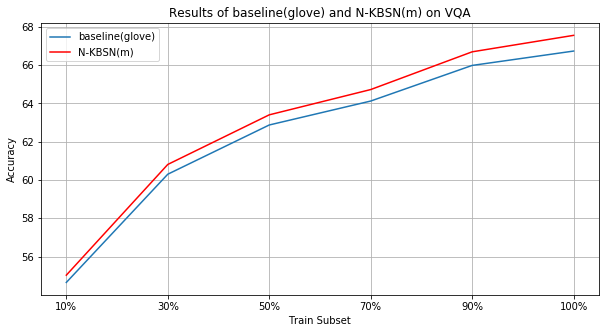
\includegraphics[width=0.8\textwidth]{subsetres_fig.png}
	\caption{$N-KBSN(m)$和$baseline(glove)$在不同训练子集的实验结果统计图}
	\label{subsetres_fig}
\end{figure}

根据上述图和表格可以看出,随着训练数据的增加,各自的准确率均单调上升,并且上升的速度逐渐趋于减小,使得准确率趋于稳定,这说明增大训练数据量能够帮助提升准确率,但是提升会趋于饱和。值得注意的是,仅仅使用10\%的训练数据,也能得到较好的准确率。

$N-KBSN(m)$的准确率始终高于$baseline(glove)$,这说明动态词向量的确能提升模型的准确率。随着数据量的增大,两个模型的准确率差值逐渐增大,我们认为这是因为动态词向量能有效表征多义词的表现,更大的训练数据意味着更有可能包含词语在不同语境的使用,静态词向量则无法有效处理这种情况。

\subsubsection{定性分析}
为了定性的分析$N-KBSN(m)$和$baseline(glove)$在验证集结果的差异,我们将两个模型在验证集的预测结果进行对比分析,以下使用$Res(elmo)$和$Res(glove)$分别代表其结果集。$Res(elmo)$和$Res(glove)$的大小均为验证集中问题的数量:214354,其中,两个模型给出不同答案的问题数为52990,约占总数的1/5。在给出的不同答案中,$Res(elmo)$答对且$Res(glove)$答错的占比为27.8\%,$Res(glove)$答对且$Res(elmo)$答错的占比为26.4\%,结果都错的比例为45.8\%,结果都对的比例为0\%,如表\ref{diff}。
\begin{table}[H]
% \resizebox{0.8\textwidth}{!}{}
\centering
\caption{$Res(elmo)$和$Res(glove)$在验证集的答案的差异。}
\begin{tabular}{cc}
\toprule
不同答案的问题数(比例) & 52,990 (24.7\%)\\
仅$Res(elmo)$答对数(比例) & 14,711 (27.8\%)\\
仅$Res(glove)$答对数(比例) & 13,991 (26.4\%)\\
都答错数(比例)& 24288 (45.8\%)\\
都答对数(比例)& 0 (0\%) \\
\bottomrule
\end{tabular}
\label{diff}
\end{table}
从总体的答案差异看,$N-KBSN(m)$答对的数量略高于$baseline(glove)$,这也符合验证集上的整体结果的表现。

我们还从答案中,挑选了一些样本来定性分析$N-KBSN(m)$优于$baseline(glove)$的可能原因,如图\ref{res_examples}。图(a)$Res(elmo)$正确识别出“浴池窗帘”的颜色,而$Res(glove)$的答案则为”白色“,我们认为这是模型错误的识别了"shower"而不是"shower curtain"的颜色。在图(b)中类似,$Res(glove)$计数对象为"people"而$Res(elmo)$则能正确的计数"elderly people"词组。图(c)则体现了$Res(elmo)$能更好的识别长句中的词组而不仅仅是识别单词的能力。
\begin{figure}[H]
	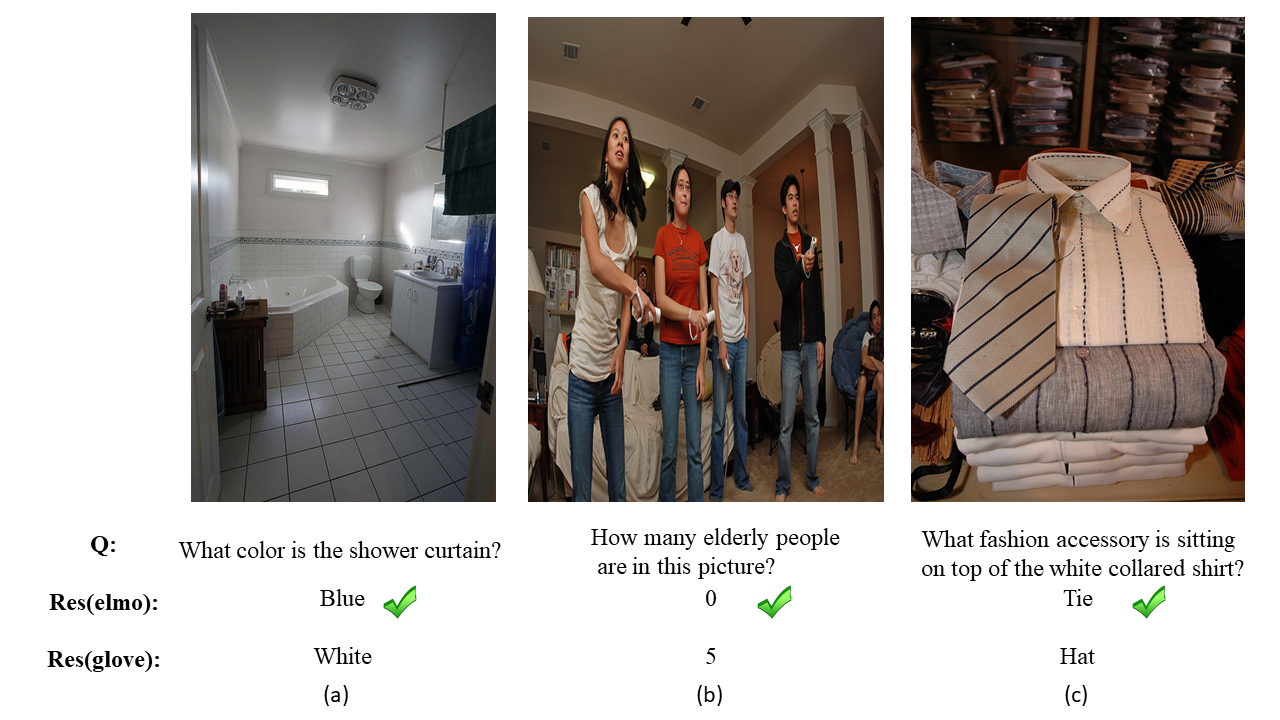
\includegraphics[width=0.8\textwidth]{res_examples.png}
	\caption{验证集的样本示例}
	\label{res_examples}
\end{figure}

\subsubsection{和已有模型的比较}
如表\ref{5mresults}所示,$N-KBSN(l)$在验证集上表现最佳,该模型和$2017-winner(glove)$和$2019-winner(glove)$在Test-dev和Test-std测试集上的结果如表\ref{testres}。测试集上的结果显示,我们提出的$N-KBSN(l)$在各项指标上均优于其他两个模型,该结果和验证集上的结果表现一致,这证明了我们改进的文本特征化方式能够提高预测的准确率。
\begin{table}[H]
% \resizebox{0.8\textwidth}{!}{}
\centering
\caption{$N-KBSN(l)$模型和其他模型在测试集上的结果对比。}
\begin{tabular}{c|cccc|c}
\toprule
\multirow{2}{*}{模型} & \multicolumn{4}{c}{Test-dev} & Test-std\\
& All & Y/N & Num & Other & All \\
\midrule
$2017-winner(glove)$ & 65.32 & 81.82 & 44.21 & 56.05 & 65.67\\
$2019-winner(glove)$ & 70.63 & 86.82 & 53.26 & 60.72 & 70.90\\
\midrule
$N-KBSN(l)$& \textbf{71.14} & \textbf{87.13} & \textbf{54.05} & \textbf{60.90} & \textbf{71.23} \\
\bottomrule
\end{tabular}
\label{testres}
\end{table}

\section{本章小结}
本章的主要内容是构建了一个基于动态词向量的联合嵌入模型(N-KBSN模型),并通过对比实验证明了动态词向量能够提高视觉问答模型的性能。

本章首先介绍了视觉问答挑战的发展情况,进一步解释了联合嵌入模型主流地位和优异表现的原因。通过对比已有代表性的联合嵌入模型,我们分析了其潜在的改进方向,从而提出了了一个基于动态词向量的联合嵌入模型——None KB-Specific Network(N-KBSN)模型。随后详细介绍了N-KBSN模型的关键部分:基于Faster R-CNN的图像特征化、基于ELMo的文本特征化和基于多头注意力机制的特征增强。

实验部分,我们使用通用的VQA2.0数据集训练和验证模型。为了探究动态词向量和静态词向量对实验结果的影响,我们固定其他模块不变,使用不同的本文特征化方法构建了多个模型。实验结果证明动态词向量的引入提高了整体结果的准确率,本文构建的N-KBSN实现了较高的预测准确率。随后,我们进一步对$N-KBSN(m)$和$baseline(glove)$进行了定性和定量分析,分析结果解释了基于动态词向量的模型整体优于静态模型的原因,也证明了引入动态词向量的有效性。



